\newsection
\section{Техническое задание}
\subsection{Основание для разработки}

Основой для разработки является задание на дипломную квалификационную работу бакалавриата "Разработка веб-сайта " veterinary clinic"на платформе Visual studio".

Некоторые из них перечислены ниже:

\begin{itemize}
 \item Определяем потребности ветеринарной клинической лаборатории: анализируем, какую информацию и услуги лаборатория хочет предоставлять пользователям на своем сайте.
\item Определите удобный и удобный дизайн: веб-сайт
Пользователям должно быть легко ориентироваться и предоставлять информацию в четкой и организованной форме.
\item Информационная безопасность: должны быть гарантированы безопасность и конфиденциальность информации, предоставляемой пациентами.
\item Обновленная информация: веб-сайт должен содержать обновленную информацию и
правдивая информация о лаборатории, предлагаемых услугах и результатах
анализ
\item  Интеграция с технологиями: следует учитывать интеграцию передовых технологий, чтобы сделать работу пользователей более приятной и эффективной, например, платформу онлайн-записи.
о пациентах, врачах и специальностях сдать результаты анализов.
\item  Сосредоточьтесь на пользовательском опыте: веб-сайт должен быть разработан
с учетом пользовательского опыта и того, как он может облегчить доступ к информации и услугам, предлагаемым клинической лабораторией.
\end{itemize}

\subsection{Цель и назначение разработки}

Веб-сайт ветеринарной клинической лаборатории предназначен для предоставления пользователям лаборатории информации о предоставляемых ею больничных услугах, а также
позволить им получить доступ к результатам тестов и контролировать лечение домашних животных.

Поэтому функция веб-сайта в ветеринарной клинической лаборатории
главным образом в облегчении доступа владельцев домашних животных и ветеринаров к информации и услугам, предоставляемым в ветеринарной клинике.

Цель и функции веб-сайта в ветеринарной клинике должны быть важными.
инструмент для быстрого и удобного доступа ко всей необходимой информации, а также облегчения
Запросить информацию и получить результаты тестирования.

С внедрением сети предполагается устранить существующие недостатки почерка и избежать потребления листов бумаги. Сайт обеспечит уверенность и безопасность в лечении пациентов.

\subsection{Требования пользователя к интерфейсу web-сайта}

Использование хорошо продуманного и простого интерфейса на сайте может обеспечить следующие преимущества:

\begin{itemize}
\item Простота использования: интуитивно понятный и простой в использовании интерфейс может помочь ветеринарам и клиентам в навигации по сайту, поиске необходимой информации и уменьшении количества сбоев.

\item Увеличьте количество пользователей: если пользователи найдут сайт простым в использовании и предоставят необходимую им информацию в ясной и краткой форме, они могут стать постоянными клиентами.

\item Ранжирование в поисковых системах: поисковые системы отдают предпочтение сайтам, которые обеспечивают хороший пользовательский опыт.

\item Повышенная безопасность: хорошо продуманный интерфейс может включать в себя меры безопасности и защиты пользователей, такие как шифрование данных и аутентификация пользователей.

\item Анализ и оценка данных: хорошо продуманный интерфейс позволяет собирать и анализировать данные об использовании страницы, что может помочь улучшить взаимодействие с пользователем и оптимизировать его.
\end{itemize}
Сайт должен включать:
\begin{itemize}
    \item навигация по разделам;
    \item авторизацию;
    \item доступно администратору, редактору, исполнителю запросов форм.
\end{itemize}

Композиция шаблона сайта представлена на рисунке ~\ref{templ:image}.

\begin{figure}[H]
\center{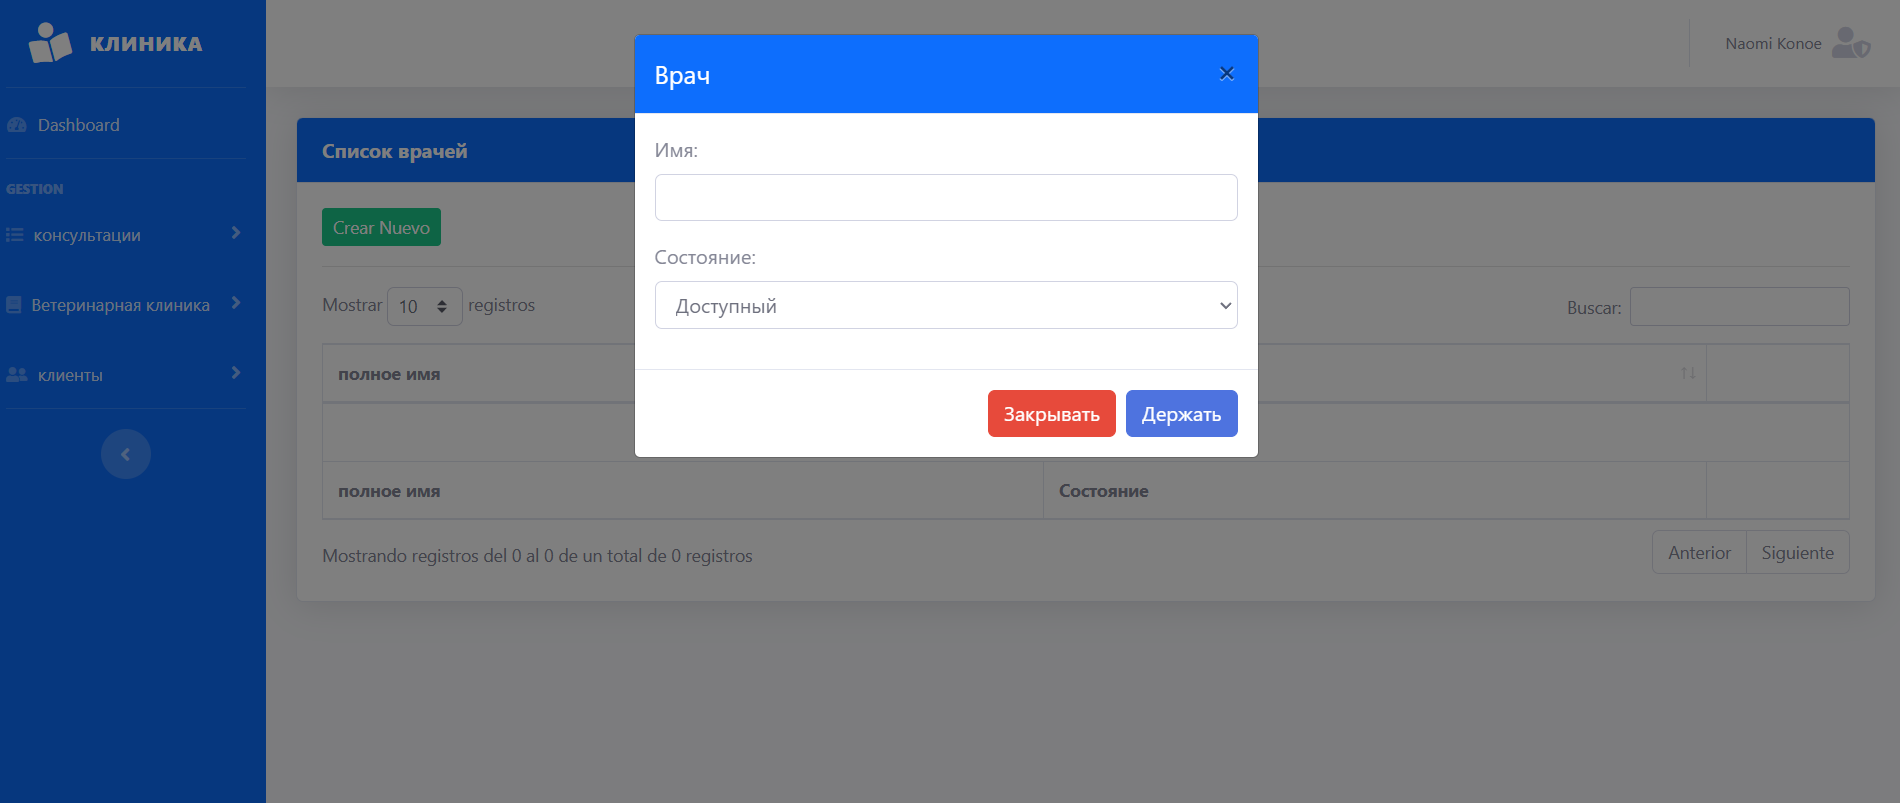
\includegraphics[width=1\linewidth]{Img 1}}
\caption{Композиция шаблона сайта}
\label{templ:image}
\end{figure}

\subsection{Требования к обработке продукции}

Модели, используемые на этом этапе, имеют дело с характеристиками системы, которые позволят ее эффективно внедрить, поэтому модули должны отвечать за конкретную задачу и быть правильно связаны друг с другом, что поможет облегчить обслуживание системы.

То есть, на этом этапе мы приступили к определению моделирования данных на основе информационной записи, которая была собрана в ветеринарной клинике, и таким образом при проектировании диаграммы базы данных можно было улучшить согласованность данных, которые должны быть сохранены. , через веб-приложение.

После того, как были проведены анализ и разработка предложения, было выполнено кодирование веб-приложения, на этом этапе могут выполняться итерации, поскольку инструмент находится в полной разработке, чтобы обеспечить полный результат для конечного продукта, поэтому что клиент может постепенно получать выгоды от проекта.

\subsection{Моделирование вариантов использования}

Для разрабатываемого сайта была реализована модель, которая обеспечивает визуальное представление вариантов использования сайта.
Помогает в разработке и детальном анализе объектных отношений. При создании диаграммы вариантов использования используется язык веб-моделирования.

Диаграмма вариантов описывает функциональное назначение разрабатываемой системы. То есть это то, что система будет делать непосредственно во время своей работы. Это исходное концептуальное представление . Проектируемая система представлена в виде серии вариантов использования, которые система предоставляет субъектам или организациям, взаимодействующим с системой. Регистратор - это организация, которая взаимодействует с системой извне (например, человек, техническое устройство.

Чтобы веб-приложение было полностью функциональным, должна быть интегрирована опция, позволяющая обслуживать все компоненты приложения, чтобы оно соответствовало всем требованиям, установленным в начале проекта, и, таким образом, инструмент был надежным и простым. использовать для конечного пользователя ветеринарной клиники.

Для поиска ошибок, которые могут появиться со временем в веб-приложении, было адаптировано использование интеграционного теста, который состоит из проверки быстрой загрузки графики и расчета времени их загрузки, что очень важно для обслуживания из любого веб-приложения.

После этого проводится Альфа-тест, который генерируется с точки зрения конечного пользователя, который, в зависимости от того, какое использование он дает приложению, определит, будет ли необходимо исправлять ошибки, модифицировать интерфейс или повысить производительность приложения веб-приложения.

Следует отметить, что данная работа не будет включать этап сопровождения как таковой, так как разработка данного проекта соответствует прототипу веб-приложения для решения задач, существующих в ветеринарных клиниках, однако основные критерии, соответствующие данному этапу проект, оставляя открытой возможность реализации и производства в будущем.

\subsection{Спецификация и функции программы}

Как указывалось ранее, веб-приложение предназначено для улучшения управления и обработки информации, чтобы административные задачи выполнялись наилучшим образом, сокращая время ожидания и улучшая обслуживание клиентов.

Это приложение имеет следующие модули:

Инвентаризация: позволяет ответственному врачу осуществлять процесс продажи и покупки, позволяет регистрировать продукты, которые продаются в ветеринарной клинике, кроме того, через список продуктов будет известно количество, доступное на складе ветеринара, что, в свою очередь, будет показать движения, сделанные для входа и выхода товара.

Назначения: позволяет планировать медицинские приемы для каждого из пациентов, принимая во внимание наличие смен и тип услуги, которая будет оказана на назначенном приеме. Следует отметить, что запись на прием может быть сделана лично в учреждении или любым пользователем, который взаимодействует с веб-сайтом.

Техническое обслуживание: позволяет отслеживать и управлять информацией, зарегистрированной в системе клиентов и пациентов, с опцией поиска, которая позволяет легко найти запрошенную информацию.

Отчеты: этот модуль позволяет владельцу клиники отображать ежемесячные продажи в числовом и графическом виде, кроме того, он позволяет экспортировать их в файлы, которые можно использовать при принятии решений в будущем.

Наконец, это приложение направлено на то, чтобы в клинике была экономическая система, адаптированная к ее потребностям и возможностям, для лучшего управления административными процессами и предоставления квалифицированных услуг, обеспечения информации и повышения лояльности клиентов.

\subsection{Требования к оформлению документации}

Разработка программной документации и программного изделия должна производиться согласно ГОСТ 19.102-77 и ГОСТ 34.601-90. Единая система программной документации.

\subsection{Стадии и этапы разработки}

Выполнение разработки должно включать три стадии:
\begin{itemize}
\item техническое задание;
\item технический проект;
\item рабочий проект.
\end{itemize}

На стадии ”Техническое задание” проводится постановка задачи, разработка требований к веб-приложения, изучение литературы по задаче и оформление документа ”Техническое задание”. На стадии ”Технический проект”проводится анализ данной предметной области, выяснение структуры программы резидента. 
В заключение данного этапа оформляется документ ”Технический проект”. На стадии ”Рабочий проект” проводится разработка схем алгоритмов для функционального модуля, физическое проектирование программного изделия, разработка тестов, тестирование программных модулей. В заключение данного этапа оформляется документ ”Рабочий проект”.
Процесс разработки веб-сайта клинической лаборатории включает несколько этапов, некоторые из которых включают следующие:

\begin{itemize}
		\item Планирование: Этот этап включает в себя определение целей веб-сайта, определение содержания и структуры веб-сайта и выявление ресурсов, необходимых для его разработки.
	
	\item Дизайн и верстка: На этом этапе создается визуальный дизайн сайта, определяется расположение элементов, разрабатывается визуальная иерархия и прорабатывается удобство использования сайта в отношении взаимодействия с врачом. 
		
	\item Определяем потребности ветеринарной клинической лаборатории: анализируем, какую информацию и услуги лаборатория хочет предоставлять пользователям на своем сайте.
	
	\item Определите удобный и удобный дизайн: веб-сайт
	Пользователям должно быть легко ориентироваться и предоставлять информацию в четкой и организованной форме.

	\item Информационная безопасность: должны быть гарантированы безопасность и конфиденциальность информации, предоставляемой пациентами.

	\item Обновленная информация: веб-сайт должен содержать обновленную информацию и
	правдивая информация о лаборатории, предлагаемых услугах и результатах
	анализ

	\item  Интеграция с технологиями: следует учитывать интеграцию передовых технологий, чтобы сделать работу пользователей более приятной и эффективной, например, платформу онлайн-записи.
	о пациентах, врачах и специальностях сдать результаты анализов.

	\item  Сосредоточьтесь на пользовательском опыте: веб-сайт должен быть разработан
	с учетом пользовательского опыта и того, как он может облегчить доступ к информации и услугам, предлагаемым клинической лабораторией.
\end{itemize}